\documentclass{beamer}
\usepackage{ctex}
\usepackage{graphicx}
\usepackage{tikz}

\title{Uniswap 简明导论}
\author{怀菁}
\institute{武汉大学}
\date{\today}

\usetheme{Madrid}


\begin{document}

\frame{\titlepage}

\begin{frame}
    \frametitle{这是什么?}

    \centering
    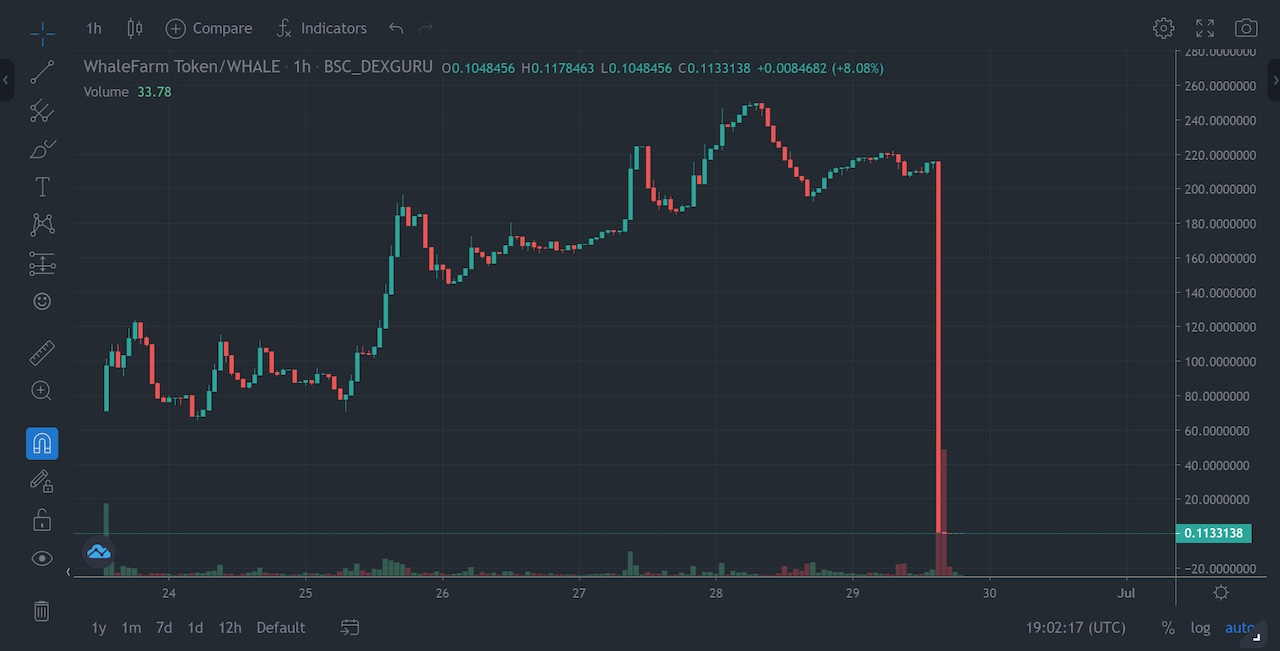
\includegraphics[width=0.8\textwidth]{../notes/rugpull.jpeg}

\end{frame}

\begin{frame}
    \frametitle{Uniswap 简介}

    \begin{itemize}
        \item 一个去中心化交易协议
        \item V1 上线时间:2018年11月2日
        \item 恒定积自动做市商
        \item 去中心化交易所的奠基者和领军者
    \end{itemize}

    ~

    \centering
    
\includegraphics[width=0.2\textwidth]{Uniswap-Logo.png}
\end{frame}

\begin{frame}
    \frametitle{中心化交易所的订单簿}

    \centering
    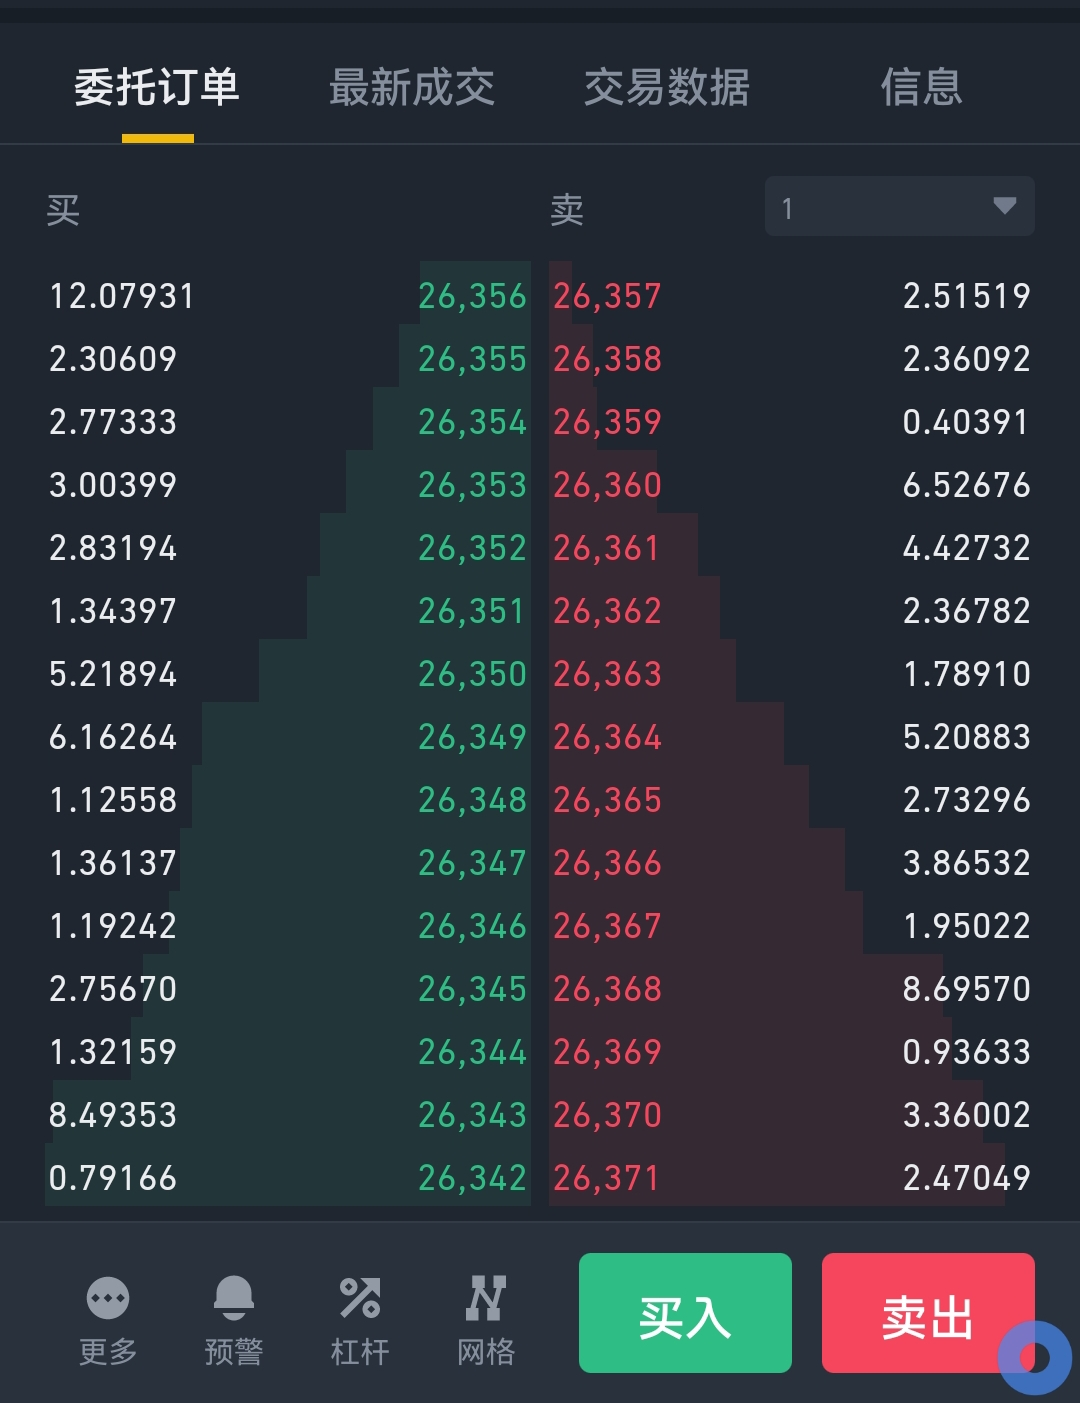
\includegraphics[width=0.5\textwidth]{../notes/订单簿示意图.jpg}
\end{frame}

\begin{frame}
    \frametitle{例子:可乐自动售货机}

    \begin{itemize}
        \item 机器中有 $x_0$ 瓶可乐与 $y_0$ 枚一元硬币
        \item 一瓶可乐 3 元
        \item 交易若干次后,机器中有 $x$ 瓶可乐与 $y$ 枚一元硬币
    \end{itemize}

    \begin{equation}
        3x + y = 3x_0 + y_0
    \end{equation}

    设 $k=3x_0+y_0$ ,有 $y=-3x+k$

    \begin{figure}[htbp]
        \centering
        \begin{tikzpicture}[scale=0.7]
            \draw[-latex] (0,0) -- (2.5,0) node[right] {$x$};
            \draw[-latex] (0,0) -- (0,4) node[above] {$y$};
            \draw[domain=0:1, thick, red] plot (\x, {-\x*3+3});
            \node[left] at (0,3) {$k$};
        \end{tikzpicture}
    \end{figure}
    
\end{frame}

\begin{frame}
    \frametitle{为可乐交易所添加流动性}

    向交易所中投放更多的可乐和硬币,得到 $k'>k$ 

    \begin{figure}[htbp]
        \centering
        \begin{tikzpicture}[scale=0.7]
            \draw[-latex] (0,0) -- (4,0) node[right] {$x$};
            \draw[-latex] (0,0) -- (0,7) node[above] {$y$};
            \draw[domain=0:1, thick, red] plot (\x, {-\x*3+3});
            \node[left] at (0,3) {$k$};
            \draw[domain=0:2, thick, blue] plot (\x, {-\x*3+6});
            \node[left] at (0,6) {$k'$};
            \draw[->] (0.5,1.5) -- (1.3,2);
        \end{tikzpicture}
    \end{figure}

    这个可乐交易所就是一个\textbf{恒定和自动做市商}(CSAMM)
\end{frame}

\end{document}